\subsection{Data Collection} 

\cite{InfosysNLP:1}For any NLP system, having a robust dataset is crucial. Data is typically split into training and testing sets. For Bengali text processing, the first step is to create a corpus of text data. Below, we demonstrate how to implement a Bengali text corpus using Python and tools such as NLTK and indic-nlp-library.

The following Python code illustrates how to process Bengali text using NLTK and indic-nlp-library for tokenization:

\begin{figure}[H]
    \centering
    \begin{subfigure}{0.6\linewidth}
        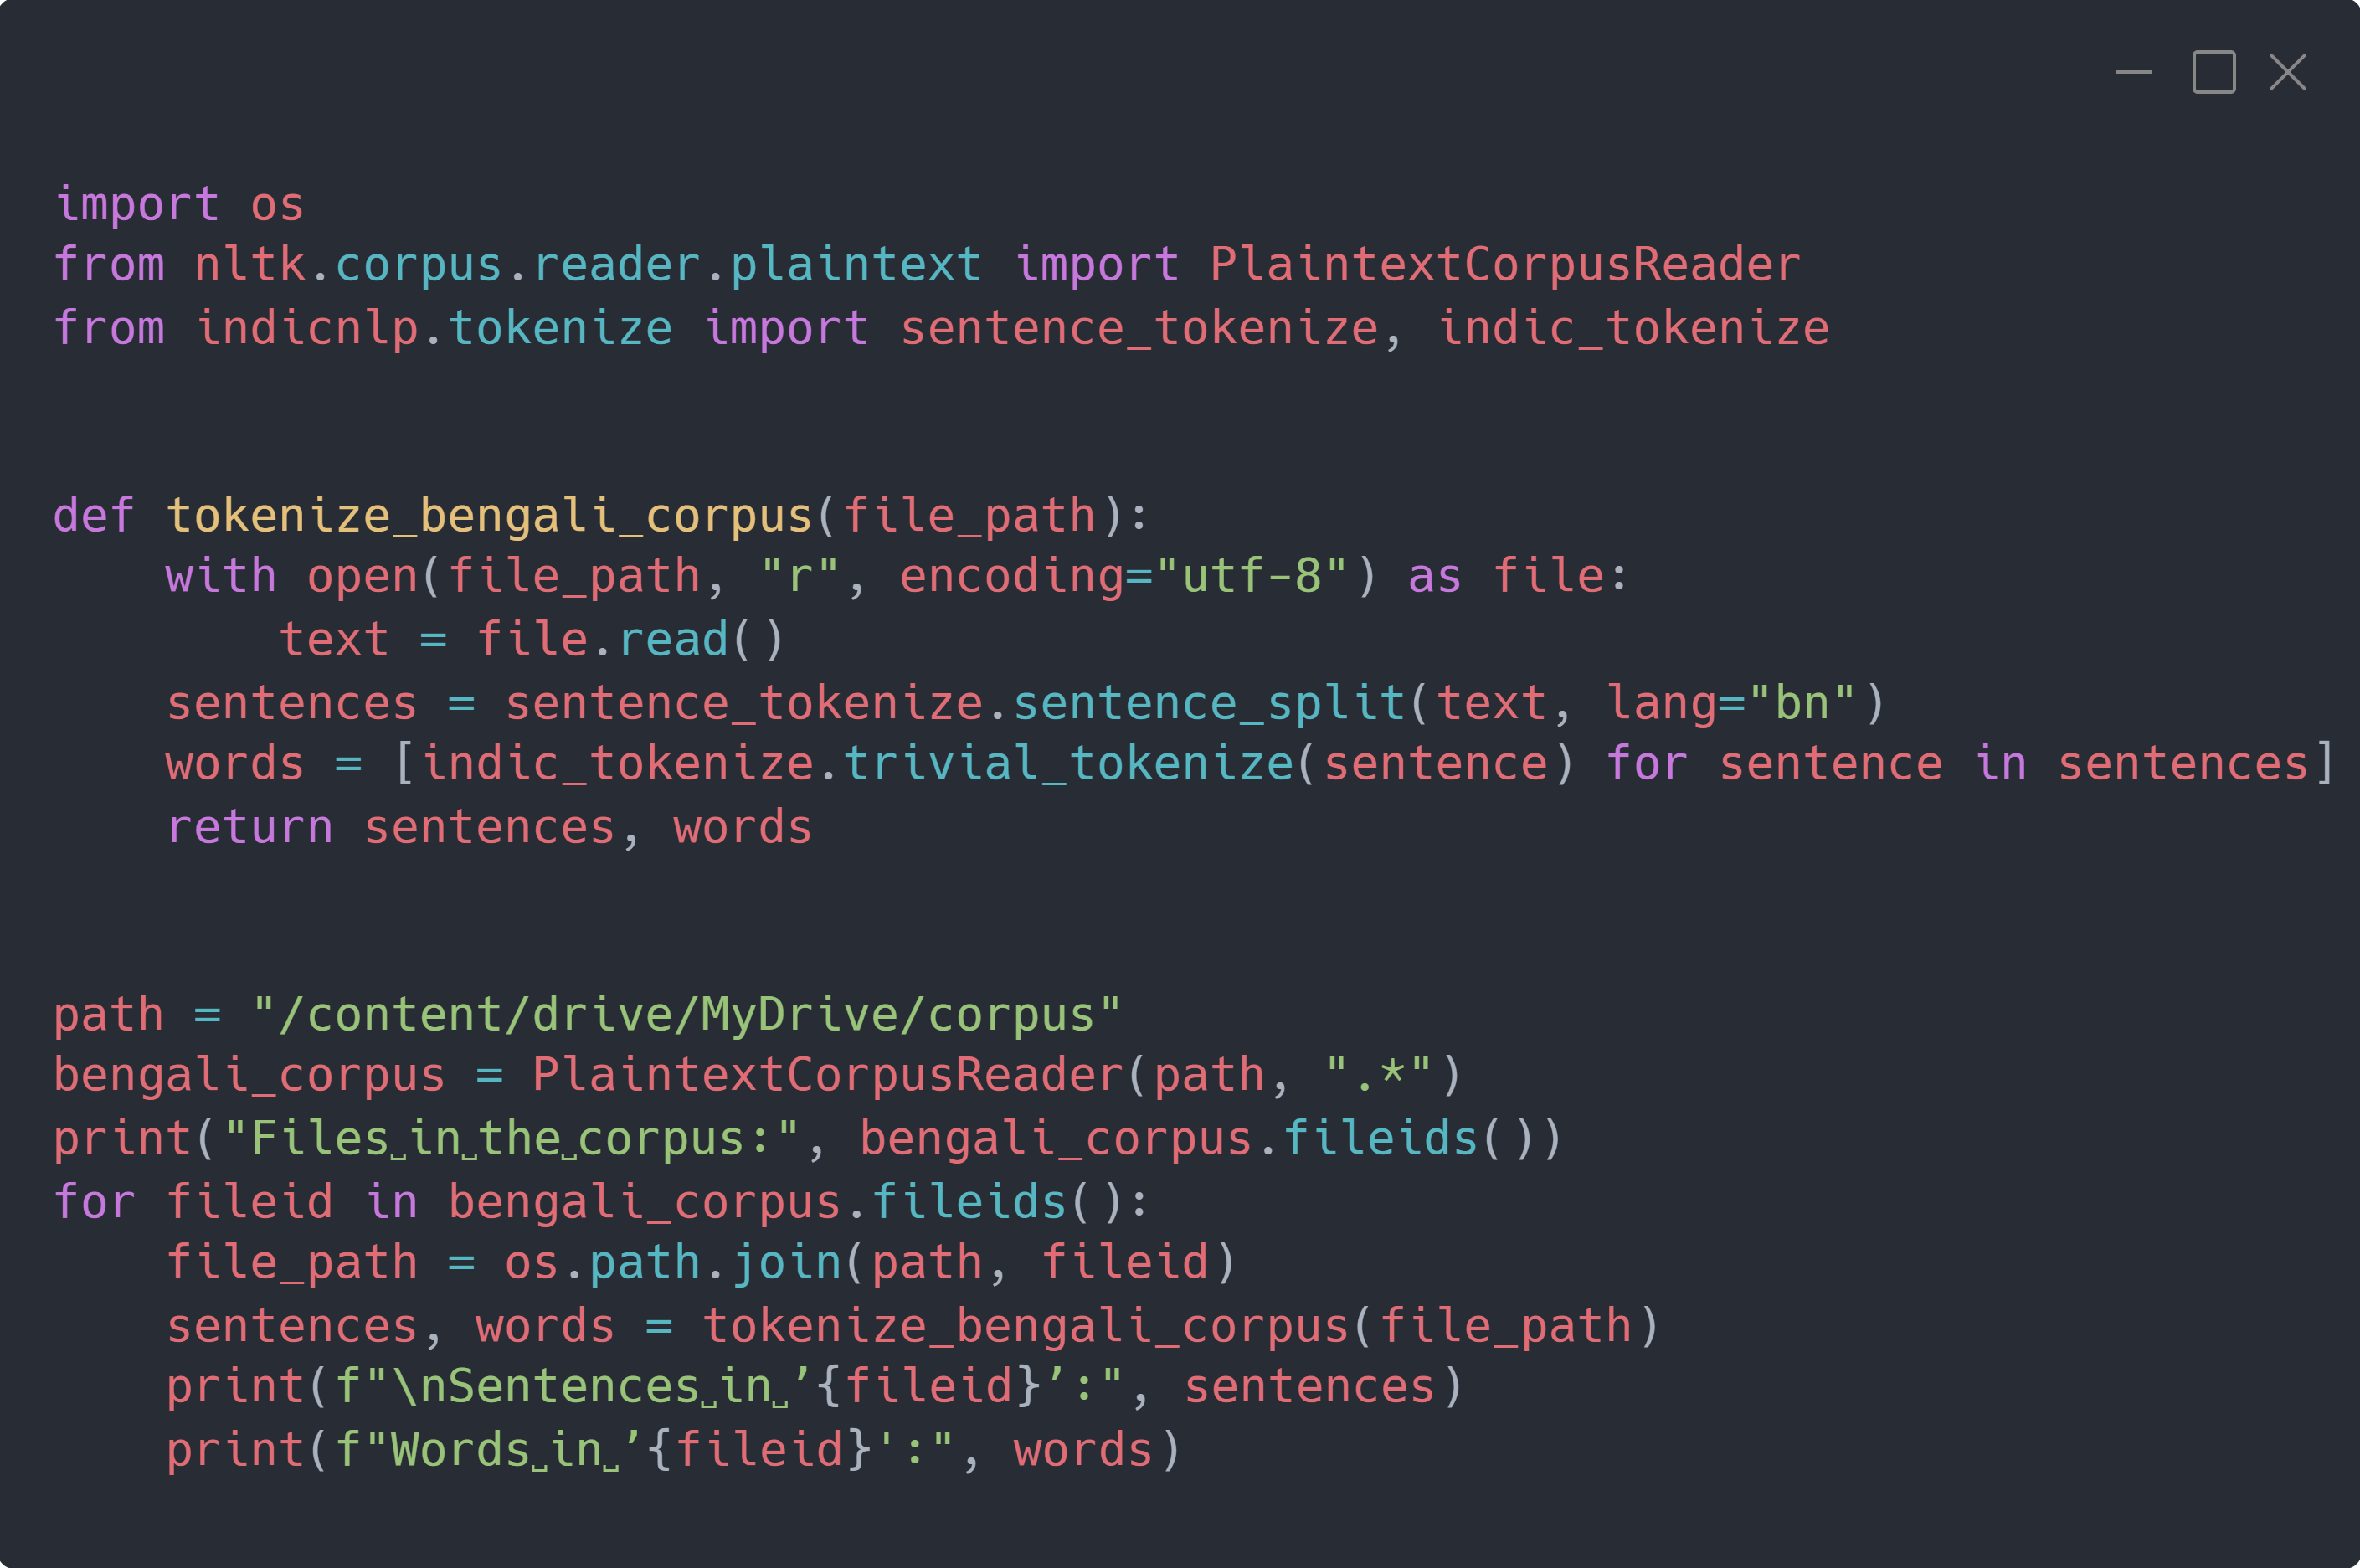
\includegraphics[width=\linewidth]{Attachments/Figures/data-collection-for-nlp_figure1.png}
        \subcaption{Source code.}
    \end{subfigure}
    \begin{subfigure}{0.6\linewidth}
        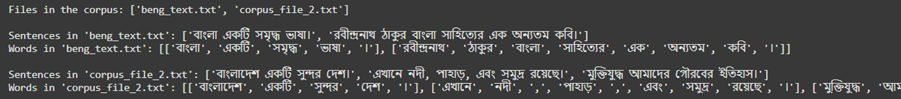
\includegraphics[width=\linewidth]{Attachments/Figures/data-collection-for-nlp_figure2.png}
        \subcaption{The terminal output of the code.}
    \end{subfigure}
    \caption{Output of the Data Collection Process.}
\end{figure}

The PlaintextCorpusReader processes the files in that directory. Sentences (sents) and words (words) are tokenized using NLTK’s default tokenizer.indic-nlp-library provides sentence and word tokenization optimized for Indic languages like Bengali.Sentences and words are tokenized properly without breaking the script.